\begin{tabular}{@{}>{\raggedright\arraybackslash}m{0.14\linewidth}m{0.105\linewidth}>{\raggedright\arraybackslash}m{0.17\linewidth}>{\raggedright\arraybackslash}m{0.08\linewidth}>{\raggedright\arraybackslash}m{0.08\linewidth}>{\raggedright\arraybackslash}m{0.08\linewidth}>{\raggedright\arraybackslash}m{0.235\linewidth}@{}}
\toprule
Outcome, question & Image & References & Correct & Partner & Unrelated & No image \\
\midrule
\textit{both right}: Does this image contain an oven? & 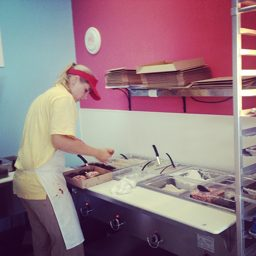
\includegraphics[height=0.46in,width=0.56in,keepaspectratio]{task2/examples/572510.jpg} & yes & yes & no & no & No, the image does not contain an oven. \\
 & 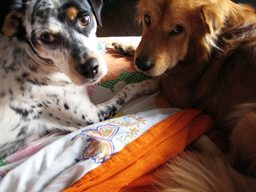
\includegraphics[height=0.46in,width=0.56in,keepaspectratio]{task2/examples/115859.jpg} & no & no & yes & no & No, the image does not contain an oven. \\ \addlinespace
\textit{identical}: Does this image contain a traffic light? & 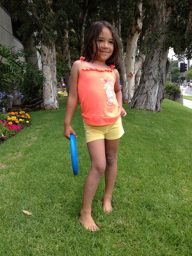
\includegraphics[height=0.46in,width=0.56in,keepaspectratio]{task2/examples/490306.jpg} & yes & no & no & no & No, the image does not contain a traffic light. \\
 & 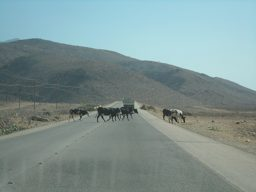
\includegraphics[height=0.46in,width=0.56in,keepaspectratio]{task2/examples/570693.jpg} & no & no & no & no & No, the image does not contain a traffic light. \\ \addlinespace
\textit{changed, not both right}: Does this image contain a handbag? & 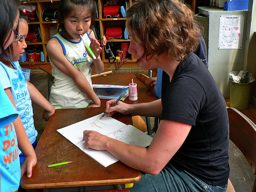
\includegraphics[height=0.46in,width=0.56in,keepaspectratio]{task2/examples/177375.jpg} & yes & no & yes & yes & No, the image does not contain a handbag. \\
 & 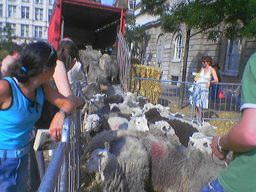
\includegraphics[height=0.46in,width=0.56in,keepaspectratio]{task2/examples/366157.jpg} & no & yes & no & no & No, the image does not contain a handbag. \\
\bottomrule
\end{tabular}